\documentclass[12pt]{article}
\pdfminorversion=7

% Standard packages for figures, citations, math, tables, etc.
% Feel free to add more as needed!
\usepackage{amssymb}
\usepackage{graphicx}
\usepackage{cite}
\usepackage[cmex10]{amsmath}
\interdisplaylinepenalty=2500 
\usepackage{mdwmath}
\usepackage{mdwtab}
\usepackage{color}
\usepackage{pgfplots}
\usepackage{multirow}
\usepackage{subcaption}
\usepackage{verbatim}
\usepackage{appendix}
\usepackage[outdir=./]{epstopdf}
\usepackage{indentfirst}
\pgfplotsset{compat=1.17}

% Packages for formatting with 1 in margins
\usepackage[latin1]{inputenc}
\usepackage[left=1in,top=1in,right=1in,bottom=1in,nohead]{geometry}
\usepackage{setspace}
\setstretch{1.15}

% Define the location of your figures in order to avoid writing absolute file location
\graphicspath{{figures/}}	

\begin{document}

% Title Page
\begin{titlepage}
\begin{center}
{\LARGE \textsc{ECE 445: Senior Design Laboratory} \\ \vspace{8pt}}
\rule[13pt]{\textwidth}{1pt} \\ \vspace{120pt}
{\huge \textbf{\textsc{The Odds Booster}} \\ \vspace{8pt}}
{\LARGE \textbf{\textsc{Project Proposal}} \\ \vspace{30pt}} 
{\large \textit{Authors:} Marco Rojas \\ \vspace{4pt}
\hspace{48pt} Jack Arndt \\ \vspace{4pt}
\hspace{48pt} Tim Green \\ \vspace{4pt}
\hspace{8pt} \textit{Date Written:} February 9th, 2022}
\vfill
\end{center}

% Numbered pages on everything but title
\pagenumbering{arabic}	
\end{titlepage}
\setcounter{page}{2}

% Body
\section{Introduction}

Before heading to the casino, individuals need to assess how much money they are willing to lose, since, as the saying goes, ``The house always wins''. Or do they? Is there potentially a way to bring the casino games to the comfort of your home and train/optimize your strategies to ask a different question, ``How much money should I win?''

The Odds Booster is an automated casino game assistant designed to help players learn and manage casino games such as Blackjack or Texas Hold'em. The kit involves a central communicable device along with a custom deck of cards which will be used to determine the best possible move for each player along with the outcome of each hand of the game. This device is an innovation as it brings both the ease and simplicity as well as the ability to learn the game that can be provided by a virtual game into the superior enjoyment and atmosphere of a physical game. Digital poker tables that provide a similar experience exist but cost thousands of dollars. Our design achieves this functionality without an expensive custom table and while allowing for physical cards and chips.

The Odds Booster central device will serve as the hub used by the dealer and all players of the game. The dealer will swipe each card being distributed to the players over the central device and said device will determine the specific card being dealt using an RFID sensor and thin passive RFID tags placed on the cards. This central device will also contain a display detailing the next actions and outcomes for each hand of the game helping each player and the dealer learn the rules of the game. This main device will be paired via bluetooth to a user's phone app. The card information will be shared with the app and the app will tell the player the strength of their hand or what move will have the best outcome within the context of the game. It is important to note that knowledge of the hands of the other players within the game provides and unfair advantage to the user and such information will be ignored when determining moves for the user. The ethics of the game will be discussed further later in this proposal. The device itself will be battery powered and rechargeable for easy use and mobility. The usage of the device is protrayed in the diagram shown in Figure \ref{fig:use_dia}.

\begin{figure}[h]
	\centering
	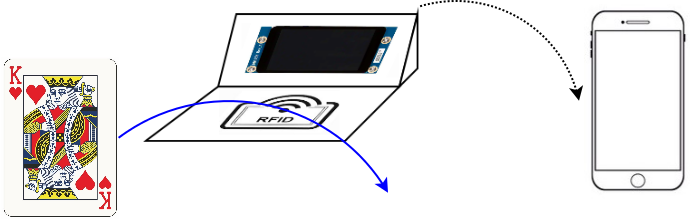
\includegraphics[width=0.98\textwidth]{ProposalUsageDiagram}
	\caption{System Usage Diagram}
	\label{fig:use_dia}
\end{figure}

\noindent
The main requirements to ensure the completion and success of this project are as follows.
\begin{itemize}
\item The central device must be able to sense and distinguish the 52 different RFID tags associated with each card and show the scanned card as well as the next action on the display.
\item The central device must be able to send game information (including cards and hands) to a phone app via bluetooth.
\item The phone app must be able to receive game information info via a bluetooth and use the information to determine the strength of the user's hand and/or the best possible move for the user.
\end{itemize}
These requirements are broken into more detailed and module specific requirements through the remainder of this proposal.

\section{Design}

words

\section{Ethics and Safety}

words

\cite{pozar}

% Bibliography (references in separate file)
\bibliographystyle{IEEEtran}
\bibliography{references.bib}

% Appendix (If Applicable)

\end{document}
